\documentclass[times, utf8, diplomski]{fer}
\usepackage{booktabs}
\usepackage{listings}
\graphicspath{{./img/}}
\lstset{language=Python, tabsize=4, numbers=left, basicstyle=\small}

\begin{document}

% TODO: Navedite broj rada.
\thesisnumber{2451}

% TODO: Navedite naslov rada.
\title{Klasifikacija pokreta ljudskog tijela temeljena na podacima s inercijskih senzora}

% TODO: Navedite vaše ime i prezime.
\author{Ivan Trubić}

\maketitle

% Ispis stranice s napomenom o umetanju izvornika rada. Uklonite naredbu \izvornik ako želite izbaciti tu stranicu.
\izvornik

% Dodavanje zahvale ili prazne stranice. Ako ne želite dodati zahvalu, naredbu ostavite radi prazne stranice.
\zahvala{}

\tableofcontents

\chapter{Uvod}
Karakteristike pokreta ljudskoga tijela vrlo su individualne te ovise o mnogo čimbenika kao što su genetika, odgoj te
fizička sprema. Ti pokreti su toliko jedinstveni da se mogu koristiti za identifikaciju osoba dok su s druge strane
toliko slični da čak i manje devijacije u tim pokretima također mogu ukazivati na neke zdravstvene probleme.
Ljudski pokreti mogu se klasificirati na razne načine koristeći računalni vid ili razne senzore postavljene na
ljudskome tijelu. Svaka od metoda ima svoju granu primjene kao: identifikacija osoba temeljenog na hodu koristeći
računalni vid na nadzornim kamerama \citep{surveillance}, pračenje pokreta igrača u interakciji sa igrama u virtualnoj stvarnosti \citep{VR},
korištenje inercijskih (IMU) senzora za precizno snimanje hoda u svhu otkrivanja bolesti i rehabilitacije te mnoge druge.

Klasifikacija pokreta vrlo je složen problem te kao takav nema dobro rješenje koristeći klasične algoritme. Razvojem moči računala
te metoda strojnoga učenja ovaj problem postaje rješiv. Za snimanje pokreta može se koristiti kamera ili senzori.
Koristeći kameru, na snimci se koriste metode računalnog vida te se traže karakteristike ljudskog tijela kako bi se na snimci
prepoznala osoba te koristeći te karakteristične točke analizira se hod. Također, kamera može snimati osobu sa posebno postavljenim
vizualnim oznakama po djelovima tijela te koristeći te vizualne oznake analizirati pokrete. Nedostatak kamera je taj što snimaju iz
jedne perspektive te zbog toga može doći do okluzije oznaka. Inercijski (IMU) senzori eliminiraju kamere te ne pate od problema okluzije.
Inercijski senzori su relativno jeftini i mali uređaji koji se postave na ključne djelove ljudskoga tijela te pružaju vrlo dobar uvid
u ljudske pokrete. Primjerice mogu se staviti na ruke te upravljati igrama i uređajima ali se mogu koristiti i u medicinske svrhe za
analizu hoda i diagnosticiranje zdravstvenih problema kao i za provođenje terapijskih vježbi bez nadzora stručnjaka.
Ovaj rad će se više fokusirati na medicinski aspekt klasifikacije pokreta, preciznije analizu hoda (\textit{eng.} gait) i terapiju koljena.



\chapter{Razrada}

\section{Bolesti koljena}

\section{Dosadašnja rješenja}

\section{Rješenje koristeći IMU senzore}

\section{Analiza IMU senzora}
IMU (eng. \textit{Inertial Measurement Unit}) je elektromehanički uređaj koji služi za mjerenje sila, kunih brzina te pozicije
uređaja koristeći skup senzora: akcelometar, žiroskop te magnetometar. Svaki od pojedinih senzora se sastoji od 3 manja senzora
koji svoj posao obavlja u odnosu na pojedinu os u prostoru. Oni u kombinaciji čine jednu jedinicu koja mjeri vrijednosti u sve 
3 prostorne dimenzije. Rane izvedbe ovakvoga senzora (poput one u Apollo 11 letjelici) su bile vrlo velikih dimenzija i nisu
u sebi imale magnetometar. Danas su se dimenzije IMU senzora znatno smanjile te je moguće izraditi sve potrebne komponente u
sklopu jednog čipa koristeći unaprijeđenja izrade sklopova u samom siliciju. Iako komponente jesu napravljene u siliciju one su
još uvijek elektromehaničke po prirodi što znači da se komponente slobodno gibaju unutar silicijske ploče na samome čipu
te su kao takve mikro-elektromehaničke (skračeno \textit{MEMS}). Danas su takvi uređaji nezamjenjivi u bilokakvim letjelicama a
pogotovo u bespilotnim letjelicama (eng. \textit{drone}) koji su u današnje vrijeme sve popularniji. Vrlo su bitni također u
navigacijskim uređajima jer u kombinaciji sa GPS uređajima daju dodatnu mogućnost pozicioniranja u slučajevima kada sam GPS signal
nije pristupačan kao što je to primjerice u tunelima te dodatno povećavaju preciznost pračenja kretanja. To je jedan od razloga
zašto je IMU senzor neizbježna komponenta pri izradi pametnih telefona. U rukama inženjera IMU senzori su dobili mnogo raznih 
kreativnih svrha te se mogu naći kao dio kontrolera u igraćim konzolama di služe kao dodatna metoda interakcije igrača sa igrom.
Prva promatrana komponenta bit će akcelometar.

\textbf{Akcelometar}

Akcelometar je senzor koji mjeri iznos sile u određenom smjeru. Jednostavan akcelometar se može konceptuirati kao masa ovješena na 
opruzi. Opruga se komprimira onoliko koliko je masa teška odnosno onoliko koliko je utjecaj gravitacije na tu masu. U slučaju
pojave nove sile u smjeru opruge ona se dodatno otpušta odnosno steže te je ukupan iznos sile na tijelo \textit{"pohranjen"}
unutar opruge odnosno istog je iznosa ali suprotne orjentacije. Kako bi se taj iznos mogao očitati u električnome obliku potrebno
je izvršiti pretvorbu a to se može ostvariti na dva načina, koristeći piezoelektrike te korištenje kapacitivnosti. Piezoelektrici
su materijali koji svoju deformaciju mogu pretvoriti u električni impuls te obratno, električni impuls mogu pretvoriti u mehaničku
deformaciju. Vrlo su korisni te njihova primjena varira od senzora koji vibracije akustičnih instrumenata pretvara u električne
signale kako bi se oni mogli snimiti i obraditi do okidača u đepnim upaljačima koji svojom deformacijom bacaju iskru potrebnu za
započimanje vatre. Od tog piezoelektričnog materijala se može napraviti opruga te bi kompresija i dekompresija opruge mogla davati
električni signal ekvivalentan iznosu sile na masu. Takva izvedba je vrlo skupa ali vrlo precizna za promatranje nekih pojava 
primjerice visokofrekventnih vibracija.

Druga mogučnost je korištenje kapacitivnosti kao mjeru kompresije i dekompresije opruge. Ako je masa ovješena na opruzi jedna ploča
kondenzatora, onda je površina na kojoj se sama opruga ovješena druga ploča kondenzatora. Ako su te dvije ploče pod naponom,
kompresija i dekompresija opruge približava i udaljava jednu ploču (masu) u odnosu na drugu ploču (površinu) te se kapacitet
povečava odnosno smanjuje što opisuje sljedeća jednadžba.

$$
C = \frac{\epsilon A}{d}
$$

Jedina promjenjiva varijabla je udaljenost $d$. Princip rada vidljiv je na slici \ref{accmtr}.


\begin{figure}[h!]
    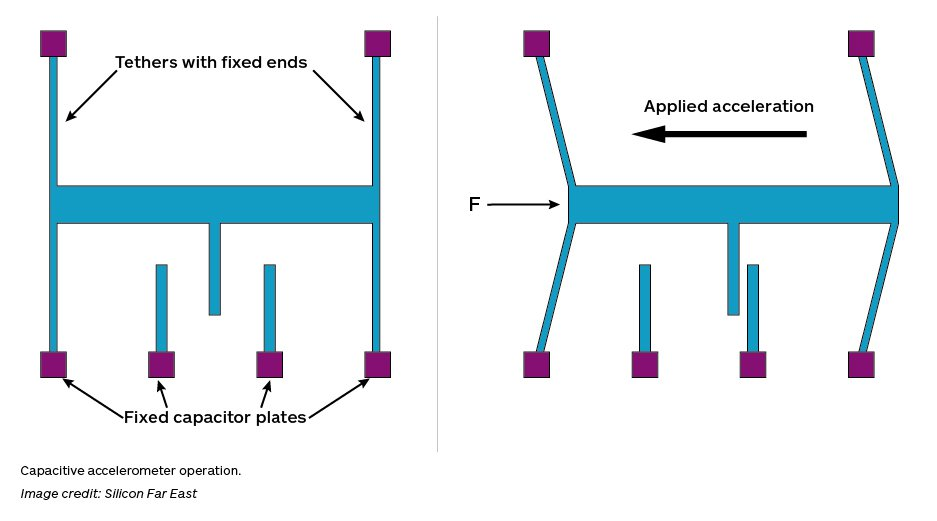
\includegraphics[width=\textwidth]{Accelerometers.jpg}
    \caption{Princip rada kapacitivnog akselometra (preuzeto sa \textit{insights.globalspec.com})}
    \label{accmtr}
\end{figure}

Kako bi se dimenzije akcelometra u potpunosti smanjile potrebno je razviti takav kapacitivni elektromehanički uređaj napravljen od
silicija koji bi bio u nekom od adekvatnih pakiranja za integrirane krugove. Također kako bi bili u mogučnosti promatrati silu u
prostoru potrebno je napraviti pojedini senzor za svaku od tri prostorne koordinate te kako bi one bile u što većoj mjeri usklađene
potrebno je sve ostvariti unutar jedne površine silicija kako bi bili skupa unutar integriranoga kruga u fiksnoj poziciji.

\textbf{Žiroskop}

Žiroskop je uređaj koji se sastoji od rotirajučeg diska koji se nalazi unutar kardanskog zgloba (eng. \textit{gimbal}). Rotirajuči
disk ima svoju kutnu količinu gibanja koja je promjenjiva jedino onda kada se na rotirajući disk djeluje silom, u protivnom
disk se rotira slobodno u ravnini u kojoj je zavrćen. Kardanski zglob je konstrukcija prstenja oko tog diska koji se oko diska
slobodno može rotirati u svim smjerovima bez da utječe na poziciju diska odnosno idejno ne djeluje silom na taj disk. Ovakav uređaj
je neznamjenjiv i jedan od najbitnijih komponenti svih letjelica jer uvijek letjelici daje referentnu točku iz koje se može
zaključiti točan položaj iste u zraku. Koristeći varijabilne otpore odnosno potenciometre postavljene na osovine kardanskog zgloba,
točna pozicija se može pretvoriti u električni signal koji se dalje može obrađivati i koristiti primjerice za
automatsku korekciju pozicije bilokakvog projektila ili letjelice koja nudi mogučnost autopilota. Također, kako je brzina prva
derivacija puta u vremenu, tako je i kutna brzina derivacija promjene kuta u vremenu te se iz brzine promjene kuta može izračunati
i kutna brzina prilikom rotacije žiroskopa. Ovakva izvedba žiroskopa je
relativno velikih dimenzija te nikako nije primjerena za ugradnju u uređaje malih dimenzija kao što je to nekakav mobilni uređaj.
Za dizajn koji je dovoljno malih dimenzija potrebno je opet okrenuti se elektromehaničkim jedinicama implementiranim u poluvodiču.
Kod takve implementacije nije moguče imati rotirajuči disk i kardanski zglob što znaći da na ovakvoj skali nije moguće ostvariti 
pravi žiroskop koji bi konstantno pratio poziciju uređaja ali je moguće napraviti uređaj koji mjeri kutnu brzinu.
Takav uređaj se sastoji od vibrirajuće strukture, pojednostavljeno dvije mase koje titraju u suprotnim smjerovima.
Prilikom rotacije, mase se više ne nalaze u inercijskom sustavu već u akceleriranome što znaći da na njih djeluju sile.
Kada je sustav u rotaciji unutar njega djeluju razne sile kao što su centrifugalna, centripetalna i Coriolisova sila.
Coriolisova sila je inercijska sila koju tijela doživljavaju prilikom gibanja u rotiranom okviru promatranja. Sveprisutna je na 
planeti Zemlji te je vidljiva prilikom puštanja značajne količine vode u umivaoniku kao smjer vrtloženja vode i zaslužna za
uragane. Smjer djelovanja Coriolisove sile je okomit na smjer gibanja te na smjer rotacijskog vektora vidljivo na slici \ref{}.

%\begin{figure}[h!]
%    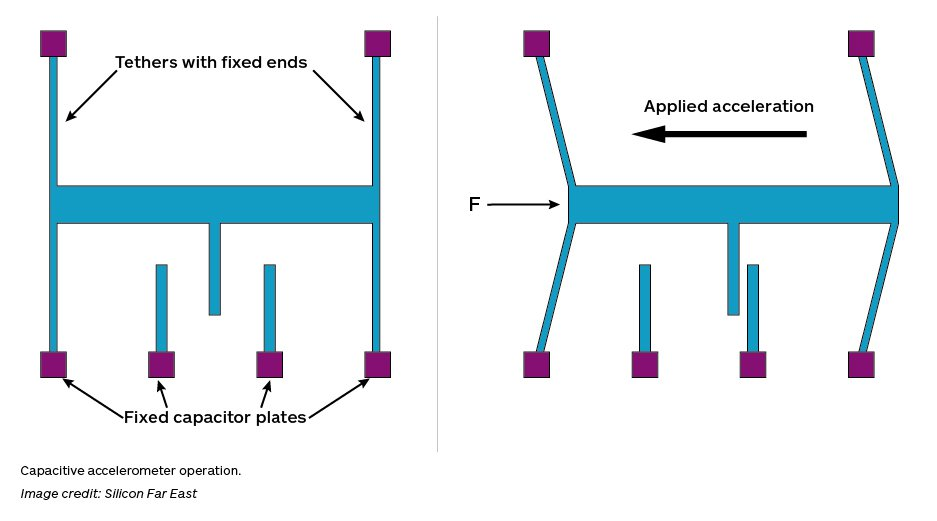
\includegraphics[width=\textwidth]{Accelerometers.jpg}
%    \caption{Princip rada kapacitivnog akselometra (preuzeto sa \textit{insights.globalspec.com})}
%    \label{accmtr}
%\end{figure}

\textbf{Magnetometar}

Magnetometar je senzor koji mjeri jačinu magnetnog polja koristeći pojave u elektromagnetizmu. Promjena magnetnog polja može
inducirati napon unutar vodića koji se nalazi u blizini no na taj se način može detektirati samo promjena. Za mjerenje magnetnog
polja koristi se Hallov efekt. Hallov efekt je fizikalna pojava koja javlja prilikom gibanja nabijene čestice kroz magnetno polje.
Električki nabijena čestica unutar magnetnog polja mjenja svoju putanju te počinje skretati i u slučaju gibanja po beskonačnoj
površini počinje svoje kružno gibanje pri čemu centripetalnu silu predstavlja Lorenzova sila. Pri ograničenoj površini nosioc
naboja putuje po vodiću prateći krivulju u smjeru u kojemu na njega djeluje Lorenzova sila te se na taj način istovrsni nosioci
nađu na istoj strani vodića te nisu nasumično raspršeni po njemu. Ta polarizacija predstavlja napon koji se može izmjeriti pri
čemu iznos tog napona ovisi o kutu između silnica magnetnoga polja i vodića te samom intenzitetu magnetnoga polja. Kako bi bi se 
nosioci naboja gibali unutar vodića potrebno je vodić spojiti na naponski izvor energije te kako bi oni imali prostora putovati na 
jednu od strana vodića on mora biti plosnat i veće površine. Primjer principa rada magnetometra vidljiv je na slici \ref{}.

%\begin{figure}[h!]
%    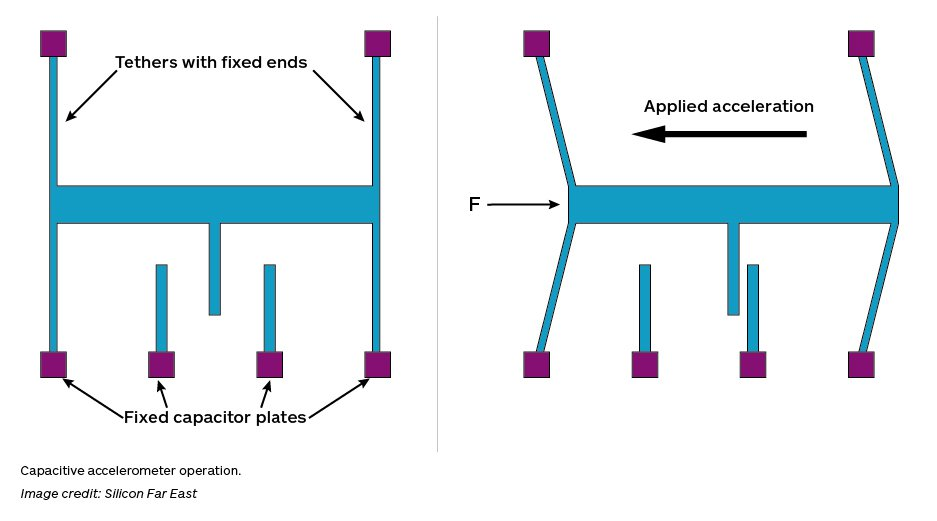
\includegraphics[width=\textwidth]{Accelerometers.jpg}
%    \caption{Princip rada kapacitivnog akselometra (preuzeto sa \textit{insights.globalspec.com})}
%    \label{accmtr}
%\end{figure}

Svaka od opisanih komponenata predstavlja samo dio pojedinog senzora i to dio koji mjeri pojave u samo jednom smjeru. Kako bi se
dobila kompletna slika potrebno je koristiti tri komponente, po jedna za svaki smjer u koordinatnom sustavu. Kako bi se to postiglo
potrebno je osmisliti arhitekturu poluvodičke pločice te paziti na preciznost i ispravno pozicioniranje svake komponente kako bi
ona mjerila točno svoj smjer u odnosu na druge. Ovakvi senzori dolaze često u pakiranju kao pojedini čipovi ili kao jedna cijela
IMU cjelina.

\section{Analiza dostupnih baza podataka}

\section{Stvaranje vlastite baze podataka}
Za stvaranje vlastite baze podataka potrebno je definirati svrhu i ciljeve te baze a zatim odrediti metodu prikupljanja podataka. U ovome će radu
fokus biti primarno na stvaranje baze podataka korisne za analizu pokreta koja bi se mogla upotrijebiti u svrhe fizikalne terapije koljena.
Za snimanje općenitih pokreta može se iskoristiti mnogo senzora postavljenih po cijelome tijelu ali za potrebe snimanja jednoga zgloba potrebno je 
koristiti dva senzora, po jedan sa svake strane uda kojeg zglob povezuje. U konkretnom primjeru koljena to su nadkoljenica i potkoljenica.

Ovisno o razini preciznosti, cjeni i dostupnosti potrebno je odabrati i same senzore za prikupljanje podataka. Redovito se sustavi senzora
za istraživačke svrhe rade baš za tu namjenu te postoji mnogo sustava otvorenog koda i otvorenih komponenti koji se mogu iskoristiti. Razni
proizvođači nude i svoja već gotova komercijalna rješenja za koje garantiraju rad i pružaju podršku ali takvi sustavi ponekad nisu adekvatni za
istraživačke svrhe zbog svoje zatvorenosti i potencijalnog manjka interoperabilnosti sa drugim uređajima i programima. U ovome radu, zbog jednostavnosti,
koristiti će se pametni telefon.

Tipičan životni vijek jednog pametnog telefona u prosjeku je dvije godine nakon čega korisnici redovito kupuju nove modele jer stariji postaju neadekvatni
po pitanju trajanja baterije, količine memorije, performansama komponenti i slično. Svaki takav stariji model telefona vrlo često stoji nekorišten iako je još uvijek
funkcionalan. Gotovo svaki pametni telefon u sebi sadrži IMU senzor te u sebi već ima povezivosti poput \textit{WiFi i Bluetooth}. Uzimajući u obzir
također da pametni telefoni imaju i ugrađenu bateriju koja može još uvijek biti dovoljno dugotrajna, ekran osjetljiv na dodir kao metodu interakcije i to 
sve ukomponirano u uređaj koji svojim dimenzijama stane u džep dolazimo do zaključka da su pametni telefoni i više nego adekvatni za prikupljanje podataka.
Također, vrlo je realna pretpostavka da svaka osoba ima pristup minimalno jednome, vjerojatno i dva pametna telefona što čini prikupljanje velike količine
podataka od većeg broja sudionika znatno jednostavnijim. Koristeći držaće pametnog telefona za trčanje ili marama, uređaji se mogu postaviti osobi na bilo koji
dio tijela vrlo jednostavno i svaka bi osoba iz svoga doma mogla pridonjeti stvaranju baze podataka.

Aplikacija koja očitava vrijednosti može biti napravljena posebno, no na tržištu postoje gotove aplikacije, redovito otvorenoga koda, koje se već time bave.
Bitno je pronaći odgovarajuću aplikaciju no u slučaju da takva ne postoji potrebno je izraditi svoju. Mnoge aplikacije u trgovini ne nude selekciju samo određenih senzora
već snimaju sve senzore kojima pametni telefon raspolaže, te u većini slučajeva nude formatiranu pohranu podataka isključivo u memoriju uređaja što je vrlo neadekvatno ako bi se uređaji
koristili primjerice za obradu informacija u stvarnome vremenu ili za centralizirano prikupljanje podataka primjerice na računalo. Neke od takvih aplikacija su
\textit{Sensor Data} i \textit{phyphox} koje se koriste u edukaciji te su u doba COVID pandemije nezamjenjivi alati za vršenje fizikalnih eksperimenata kao dio
školske zadaće. Nedostatak ovih aplikacija je taj što sve podatke snimaju na lokalnoj memoriji uređaja te nisu primjerene za obradu podataka u stvarnome vremenu.
Aplikacija \textit{Sensorstream IMU+GPS} ne nudi grafičke prikaze podataka već u svojoj vrlo bazičnoj funkcionalnosti nudi odabir senzora uz prikaz trenutnih
vrijednosti istih te odabir akcije koju želimo napraviti sa tim podacima. Ponuđene su funkcije spremanja vrijednosti u CSV (\textit{Comma separated value}) formatu,
slanje podataka koristeći UDP protokol te kombinaciju oboje. Za slanje podataka korištenjem UDP protokola potrebno je navesti određenu IP adresu uređaja te \textit{port} na
kojemu uređaj očekuje promet. Također nudi 4 frekvencije uzorkovanja označene sa \textit{slow, medium, fast i fastest}. Te frekvencije uzorkovanja nisu dobro dokumentirane
te nigdje nije navedeno koliko one iznose zapravo. Za mjerenje tih frekvencija može se iskoristiti alat \textit{wireshark}. Wireshark je alat otvorenoga koda koji
služi za analizu mrežnoga prometa. Vrlo raširen i nezamjenjiv alat za svaku granu računarstva koja se bavi mrežnim prometom. Nudi razne opcije od kojih je jedna 
od močnijih ugrađeni filter koji vrlo precizno može naći određeni paket unutar snimke mrežnog prometa. Koristeći tu mogučnost promet se može snimiti na računalu
te kasnije filtrirati samo one pakete koje mobilni uređaj šalje. Gledajući vremenske indekse prvoga i posljednjega paketa dobivamo ukupno trajanje
snimanja te znajući točan broj paketa može se izračunati približna frekvencija uzorkovanja te su one prikazane u tablici \ref{frekvencije}.

\begin{table} [h!]
 \centering
    \begin{tabular}{|c|c|c|c|}
        \hline
        Uzorkovanje & Trajanje (s) & Broj poruka & Frekvencija \\
        \hline
        Slow & 12.21 & 61 & 5 \\
        Medium & 3.98 & 61 & 15 \\
        Fast & 6.85 & 344 & 50 \\
        Fastest & 2.14 & 299 & 124\\
        \hline
    \end{tabular}
    \caption{Izmjerene frekvencije uzorkovanja}
    \label{frekvencije}
\end{table}

Također koristeći wireshark alat može se jedan paket analizirati i vidjeti format podataka koju uređaj šalje. Podaci su u CSV formatu u kojima se šalje vremenski indeks,
identifikacijski brojevi senzora te same vrijednosti senzora kako se vidi u slici \ref{datagram}. Svi podaci prikazuju vrijednosti redom $x$, $y$, i $z$ osi.

\begin{figure}[h]
    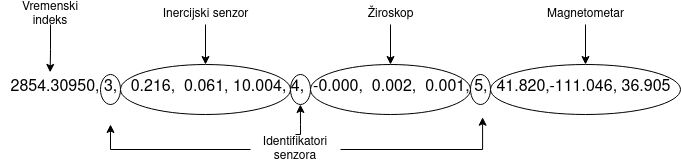
\includegraphics[width=\textwidth]{datagram.png}
    \caption{Primjerak primljenih podataka}
    \label{datagram}
\end{figure}

Kako bi se ti podaci primili i pohranili na adekvatan način potrebno je napraviti program klijent koji osluškuje na određenim portovima. Implementacija tog programa 
u ovome radu biti će napravljena koristeći skriptni jezik python. 

Python je vrlo popularan jezik mnogih mogučnosti koji je vrlo jednostavan za naučiti i koristiti te zbog svoje popularnosti raspolaže mnogim bibliotekama.
Neke od tih vrlo korisnih biblioteka koje će biti korištene u ovome radu su \textit{numpy}, \textit{matplotlib} te \textit{socket}. Python se kao skriptni jezik
izvodi liniju po liniju te se svaka linija iterpretira tek kad ona dođe na red za izvršavanje što ukida proces prevođenja programa u strojni kod kao što je to primjerice
potrebno kod programskog jezika \textit{C}. Iz tog razloga je vrijeme izvršavanja takvoga koda znatno dulje što znatno utječe na performanse programa. Kako bi se
izvođenje kompliciranijih matematičkih operacija znatno ubrzalo te kako bi se ponudio veći opseg već gotovih funkcija napravljena je biblioteka \textit{numpy}.
Numpy je biblioteka koja nudi gotovo sve potrebne funkcije za izradu programa koji se koriste u znanosti. Implementira višedimenzionalne matrice te sve funkcije
za operaciju nad njima uključujući promjenu oblika matrice te sve matrične operacije. Također nudi i funkcije za Fourierovu transformaciju, statističku obradu,
generatore nasumičnih brojeva i slično. Numpy implementacija matrica je znatno bliža onakvim matricama kao što su u programskome jeziku C te su kao takve memorijski
znatno manje zahtjevne od originalnih matrica koje nudi python. Također kako bi operacije nad matricama bile brze operacije su implementirane u programskome jeziku C te
prevedene unaprijed tako da biblioteka nudi vrlo jednostavnu sintaksu uz jako veliku brzinu izvođenja te manju veličinu datoteke pri pohrani podataka.
Biblioteka \textit{socket} nudi funkcije za umreživanje koje su potrebne kako bi se podaci uspješno primili sa mobilnih uređaja je \textit{matplotlib} koji je potreban
za vizualizaciju podataka u obliku grafova.

\begin{lstlisting}[caption=Ostvarivanje veze na strani klijenta, label=socket]
def init_client(srv_port):
    client_socket = socket.socket(family=socket.AF_INET,\\
                                    type=socket.SOCK_DGRAM)
    client_socket.bind((self_ip, srv_port))
    return client_socket

client = []

client.append(init_client(port))
print("UDP client up") 
\end{lstlisting}

U kodu \ref{socket} je vidljiv način na koji se koristi biblioteka \textit{socket}. Svaki mobilni uređaj predstavlja instanca klase \textit{socket} koja se sprema
u listu klijenata \texttt{client} što omogučuje povezivanje proizvoljnog broja mobilnih senzora pri čemu svaki senzor treba imati svoj poseban port. Port na računalu
bi trebao biti slobodan odnosno niti jedna druga aplikacija ne bi smjela koristiti taj port za svoj promet. Dobra praksa nalaže da se za osobne potrebe koriste portovi
brojeva većih od 1024 kako bi se izbjegli moguči zauzeti portovi nekakvih standardnih protokola kao što su \textit{https} i slični. U ovome slučaju mobilni uređaj
s indeksom 0 koristi port broja 5555 te svaki sljedeći zauzima port $5555 + i$ pri čemu je $i$ indeks uređaja. Točan broj je potrebno unjeti ručno na svaki uređaj
koji šalje podatke. Stvaranje instance \textit{socket} odvija se u liniji 2 i 3 pri čemu se u argumentu treba navesti tip veze. Za familiju veze se navodi
\texttt{AF\_INET} što predstavlja IP protokol te pod tip se navodi \texttt{SCOK\_DGRAM} što označava korištenje UDP protokola. UDP (eng. \textit{User Datagram Protocol})
je jedan od osnovnih transportnih protokola koji podatke prenosi po principu \textit{best effort}, pretpostavlja se da su datagrami došli do odredišta u ispravnome redosljedu
te se ne potvrđuje primitak datagrama. Ovakav protokol ne garantira cjelovitost podataka no nudi manje zagušenje prometa zbog nedostatka potvrđivanja svakog primljenog
datagrama i retransmisije u slučaju gubitka te se iz tog razloga koristi za prijenos videa ili VoIP (eng. \textit{Voice over IP}) pozive. U liniji 4 se instanca razreda
\textit{socket} povezuje s odgovarajučim portom na odgovarajučem mrežnom uređaju koji je predstavljen vlastitom IP adresom \texttt{self\_ip}. Na kraju funkcija
\texttt{init\_client} vraća instancu kako bi bila spremljena u klijentsku listu.

\begin{lstlisting}[caption=Primanje podataka, label=primanje]
while(True):
    sample = []
    for phone in client:
        bytes_adress_pair = phone.recvfrom(buffer)
        data = []
        message = bytes_adress_pair[0].decode().split(",")
        for i in message:
            data.append(i.strip())

        # filteri podataka
        if "4" not in data:
            continue

        for i in data_filter:
            data.pop(i)
        
        if len(data) != 0:
            sample.append(data[:6])
            
    if len(sample) != 0:
        signal.append(sample)
    else:
        continue
\end{lstlisting}

U odsječku koda \ref{primanje} prima se datagram svakog mobilnog uređaja. Svaki datagram se uzima iz međuspremnika koji je veličine 1024 bajta. Svaki datagram se sastoji
od samih podataka (u 6. liniji koda pod indeksom 0) te IP adrese pošiljatelja koja u ovoj implementaciji nije potrebna te se može izostaviti. Nad podacima se vrše obrade
poput uklanjanja bjelina (linija 8.) te rastavljanje podataka iz jednog monolitnog zapisa podataka u više posebnih podataka pomoću \texttt{split} funkcije uzimajući
zarez kao graničnik. Zatim te podatke valja filtrirati pri čemu se uklanja \textit{vremenski indeks}, identifikatori senzora te podaci magnetometra
vidljivi na slici \ref{datagram}. Eksperimentalno se pokazalo da se pri prvih nekoliko mjerenja od početka slanja podataka sa mobilnih uređaja izostavljaju vrijednosti
žiroskopa te se gledajući prisutnost tih vrijednosti dodatno vrši čekanje na spremnost svih senzora u mobilnome uređaju. U ovome kodu to se vrši uvjetovanjem u liniji 11.
Struktura podataka je prikazana u slici \ref{struktura}.

\begin{figure}[h]
    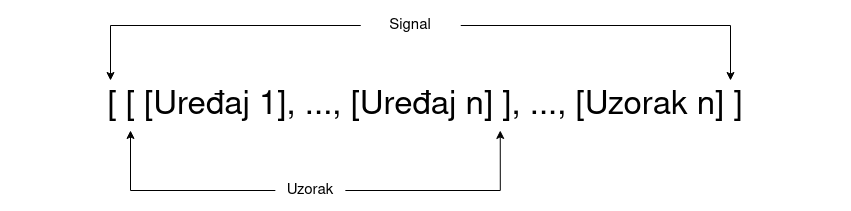
\includegraphics[width=\textwidth]{OrganizacijaPOdataka.png}
    \caption{Struktura podataka}
    \label{struktura}
\end{figure}

Uzorak jednoga uređaja je lista vrijednosti njegovih senzora. Jedan uzorak je lista uzoraka \textbf{svih} uređaja. Signal je samo lista uzoraka. Na ovaj se način akcija 
može snimiti i koristeći biblioteku \textit{numpy} pohraniti na računalo za daljnju obradu.

Kako bi se prikupili odgovarajući podaci za treniranje i uporabu neuronske mreže potrebno je iz toka podataka izdvojiti pojedina ponavljanja vježbi kako bi samo ti bitni
segmenti ili bili prikupljeni za treniranje neuronske mreže ili kako bi se pojedini segment predao neuronskoj mreži na klasifikaciju. 
Mnogi radovi primjerice \cite{android}, \cite{exo} i \cite{LowerLimb} spominju pronalazak karakterističnih točaka unutar signala
kao jednu od glavnih faza predobrade signala. Ovisno o željenom rezultatu moguće je promatrati statičke osobine signala
kao što su to prosjek, standardna deviacija, variancija i slično te dinamičke kao što su to energija, prosjek energije, odnos
harmonika, energetska entropija i slično \citep{android}. Također je moguće napraviti posebne klasifikatore koji su u suštini
neuronske mreže trenirane posebno za detekciju pojedinih osobina signala kao što su to napravili \cite{exo}. 
Najjednostavniji pristup tome je promatranje samo jedne osi određenoga senzora u nekome vremenskom periodu kao što su to napravili
\cite{LowerLimb}. Promatranjem samo jedne osi jednoga senzora fokus može biti na pseudoperiodičnosti tog signala te se detekcija
periodičnosti i segmentacija može odviti pomoću detekcije rubnih vrijednosti. Izvođenjem jednostavnije vježbe poput ispruživanja
potkoljenice (eng. \textit{leg extension}) s obzirom na poziciju mobilnog uređaja koji se nalazi ekranom okrenutim od potkoljenice uspravno na
potkoljenici može se sav fokus staviti na vrijednosti žiroskopa u $x$ osi. Snimajući te iscrtavajući odgovarajuče vrijednosti
na grafu vrlo je jasno vidljiv period te same karakteristike funkcije (slika \ref{period}). Dok se vježba ne izvodi signal je
vrlo miran i iznosi približno 0. U trenutku početka pružanja potkoljenice zbog smjera rotacije mobilnog uređaja kutna brzina iznosi
otprilike $-2.5 rad/s$. Zatim se potkoljenica u stanju potpune ispruženosti smiri te kutna brzina iznosi 0. Pri spuštanju kutna
brzina raste te također iznosi približno $2.5 rad/s$, ali u ovom slučaju u pozitivnom smjeru. Uzeći ove vrijednosti može se ostvariti
konačan automat koji prati vrijednosti signala te mjenja stanja u odnosu na iste pri čemu se pamti početak perioda. Ako se automat nađe u
prihvatljivom stanju onda to predstavlja kraj periode te je poznat cijeli segment signala koji predstavlja jedno ponavljanje.

\begin{figure}
    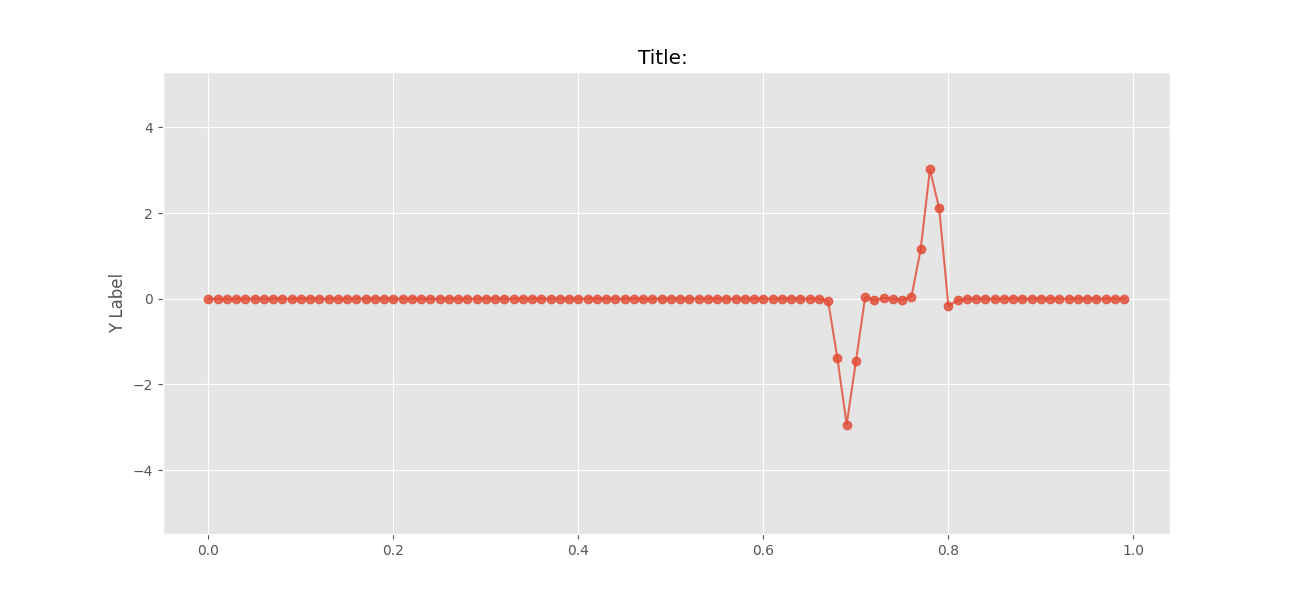
\includegraphics[width=\textwidth]{period.png}
    \caption{Primjer jednog ponavljanja vježbe, x - vrijeme, y - kutna brzina}
    \label{period}
\end{figure}

\section{Implementacija metode strojnoga učenja}

\section{Rezultati}

\chapter{Zaključak}
Zaključak.

\bibliography{literatura}
\bibliographystyle{fer}

\begin{sazetak}
Sažetak na hrvatskom jeziku.

\kljucnerijeci{Ključne riječi, odvojene zarezima.}
\end{sazetak}

% TODO: Navedite naslov na engleskom jeziku.
\engtitle{Title}
\begin{abstract}
Abstract.

\keywords{Keywords.}
\end{abstract}

\end{document}
